\chapter{RELATED RESEARCH}

\section{GPS}
GPS guidance systems are one of the most reliable guidance systems. There are many advantages to GPS, such as low cost, portability, and able to work anywhere without any pre-installation. However, the accuracy of GPS has always been a problem for agriculture. An experiment in 2014 found that 
\begin{quote}
\textit{almost half (49.6\%) of all ≈68,000 GPS points recorded with the Qstarz Q1000XT GPS units fell within 2.5 m of the expected location, 78.7\% fell within 10 $m$ and the median error was 2.9 $m$. The four different types of areas showed considerable variation in the median error: 0.7 $m$ in open areas, 2.6 $m$ in half-open areas and 5.2 $m$ in urban canyons.} \cite{schipperijn2014dynamic}
\end{quote}
According to this research, the median error for GPS is 0.7 $m$ in open areas, which is 70 $cm$. This accuracy is obviously not enough for field operations because row spacing is 76.2 $cm$.

\section{Improved GPS guidance}
An improved technology for GPS, CP-DGPS (Carrier Phase Differential GPS) or RTK GPS (Real-Time Kinematic GPS), brought the accuracy to centimeter level. This RTK GPS has two receivers; one is called \textit{reference}, while another is called \textit{rover}. \textit{Reference} is a receiver that is installed to a fixed position, which is the base station in Figure 2.1. It always stays at the same position and permanently receives satellite signals, calculates its ‘GPS’ position and determines the difference with the coordinates attributed to its own position. The \textit{rover} is mobile and placed where it is needed. It receives both GPS signals from satellites and the correction values from the \textit{reference} via radio signals. The accuracy of RTK GPS is around 2-3 $cm$. \cite{lambiel2004contribution} However, the ground condition of crop fields is unpredictable, so the 2-3 $cm$ accuracy for GPS does not equate to 10 $cm$ accuracy for tractors. It is infeasible for the large tractor to do centimeter-level adjustment.
\begin{figure}[ht!]
\begin{center}
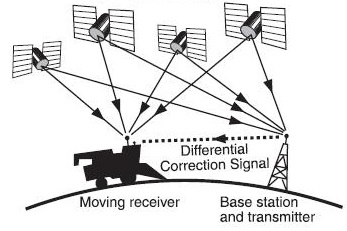
\includegraphics[scale = 1.1]{pics/RTGPS.jpg}
\caption{Real-Time Differential GPS}
\end{center}
\end{figure}
In fact, the error is about 10 $cm$ based on an experiment with a large farm tractor. \cite{thuilot2002automatic} 
%This error is acceptable with most popular 76.2 $cm$ row spacing now, but not for the 50.8 $cm$ or 38.1 $cm$ row spacing in the future. \cite{fawcett2014farm} 

\section{Vision-Based Guidance}

Vision-based guidance is an efficient way to improve the actual accuracy and lower the cost of using precision GPS. There are two methods; 3D imaging and color detection. They are both limited. The 3D imaging method detects the height of crops, so it cannot work on young crops. The color detection method finds the color of crops. However, the color of crops may vary from crop to crop and season to season. A recent study introduced a new method called image processing. The new algorithm uses the parallel texture of crop rows as the reference. \cite{english2014vision} (Figure 2.2)

\begin{figure}[ht!]
\begin{center}
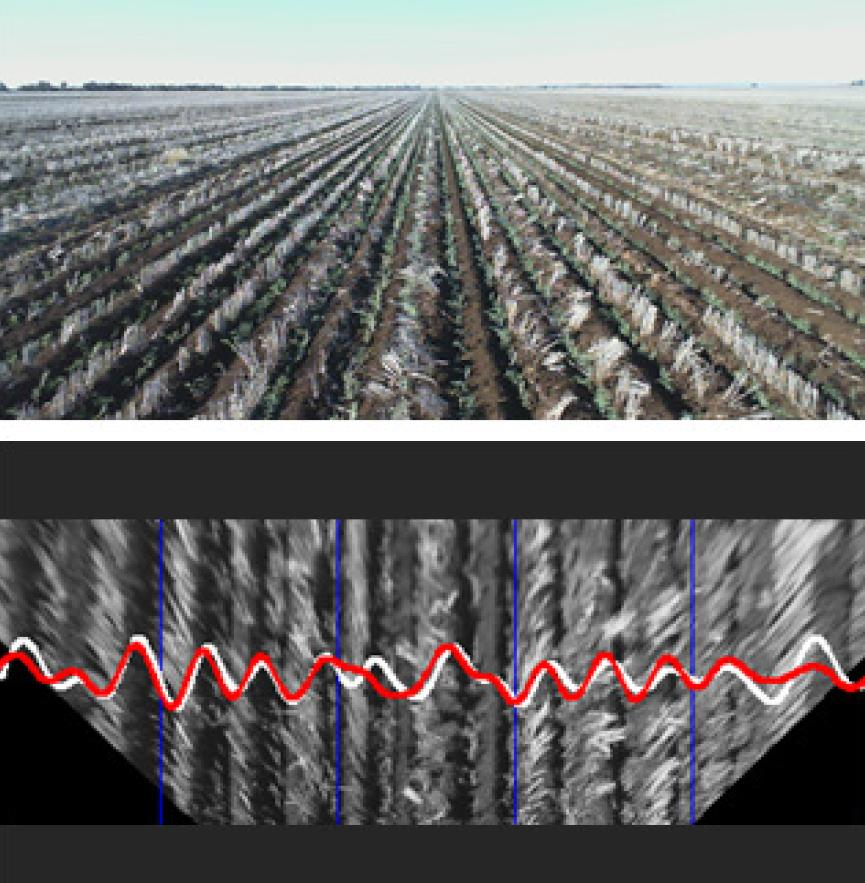
\includegraphics[scale = 0.5]{pics/parallel.jpg}
\caption{Parallel Texture}
\end{center}
\end{figure}

The result shows the accuracy is mostly lower than 10 $cm$. Therefore, this low-cost, vision-based guidance may be a very competitive alternative solution to precision GPS in the future. However, there is one fatal flaw: it needs nice parallel rows to work. It is difficult for a tractor, even with precision GPS, to create these parallel rows because  GPS-guided tractors do not compensate for sliding and tilt.

\begin{quote}
\textit{The wheat and chickpeas datasets shows the least offset error which we attribute to the narrow spacing and relatively clear crop template.}

\textit{The largest diversion at around 300m occurs while the robot is driving at an angle over a contour bank (raised ridge for diverting water). The rows are likely to not have been straight in this location since GPS guided tractors commonly do not compensate for the tilt of the vehicle as they drive at an angle over contour banks causing the planted rows to wobble.}
\end{quote}

\section{Sliding Correction}
Unlike asphalt roads, soil cannot provide constant friction on each tire of a vehicle. Sliding is a significant problem that causes trajectory errors. Therefore an algorithm for sliding estimation was developed. Two inclinometers were installed on the vehicle to collect data. (Figure 2.2) 
\begin{figure}[ht!]
\begin{center}
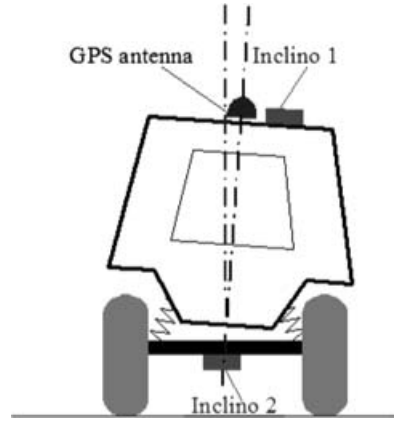
\includegraphics[scale = 0.5]{pics/slidingcorrection.png}
\caption{Position of Inclinometers}
\end{center}
\end{figure}
From these two tilt angles, the design algorithm can estimate the sliding and then give feedback to the control system for correction. The result from this research is shown in Table 2.1. \cite{lenain2006high}
\begin{table}[ht!]
\begin{center}
\caption{Deviation Signal Properties}
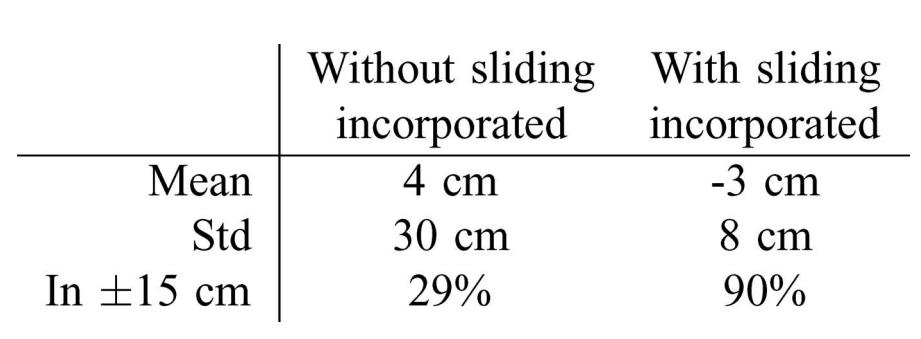
\includegraphics[scale = 0.5]{pics/slidingresult.jpg}
\end{center}
\end{table}